\section{Phân tích và Thiết kế hệ thống}
\label{chap:phan_tich_thiet_ke}

\subsection{Mô tả Dữ liệu}
Đề tài sử dụng bộ dữ liệu Book-Crossing \cite{dataset} (đã được rút gọn cho mục đích demo) gồm 3 file. Dữ liệu gốc sử dụng dấu chấm phẩy (;) làm phân tách.

\textbf{books.csv}
Chứa thông tin về sách. Dữ liệu demo gồm 5 cuốn sách.
\begin{table}[H]
    \centering
    \caption{Mô tả file books.csv}
    \begin{tabular}{|l|l|l|}
    \hline
    \textbf{Tên cột} & \textbf{Kiểu dữ liệu} & \textbf{Mô tả} \\ \hline
    ISBN & String & Mã định danh sách (Khóa chính) \\
    Book-Title & String & Tên cuốn sách \\
    Book-Author & String & Tên tác giả \\
    Year-Of-Publication & Int & Năm xuất bản \\
    Publisher & String & Nhà xuất bản \\
    ... & String & Các cột URL hình ảnh \\ \hline
    \end{tabular}
\end{table}

\textbf{users.csv}
Chứa thông tin người dùng. Dữ liệu demo gồm 5 người dùng.
\begin{table}[H]
    \centering
    \caption{Mô tả file users.csv}
    \begin{tabular}{|l|l|l|}
    \hline
    \textbf{Tên cột} & \textbf{Kiểu dữ liệu} & \textbf{Mô tả} \\ \hline
    User-ID & Int & Mã định danh user (Khóa chính) \\
    Location & String & Địa điểm \\
    Age & Int & Tuổi (NULL được xử lý) \\ \hline
    \end{tabular}
\end{table}

\textbf{ratings.csv}
Chứa thông tin rating (ma trận thưa). Dữ liệu demo gồm 10 rating.
\begin{table}[H]
    \centering
    \caption{Mô tả file ratings.csv}
    \begin{tabular}{|l|l|l|}
    \hline
    \textbf{Tên cột} & \textbf{Kiểu dữ liệu} & \textbf{Mô tả} \\ \hline
    User-ID & Int & Mã định danh user \\
    ISBN & String & Mã định danh sách \\
    Book-Rating & Int & Điểm đánh giá (0-10) \\ \hline
    \end{tabular}
\end{table}

\subsection{Luồng xử lý tổng quan của hệ thống}
Hệ thống được thiết kế theo 4 bước chính, tuân thủ kiến trúc phân tích Big Data điển hình:

\begin{figure}[H]
    \centering
    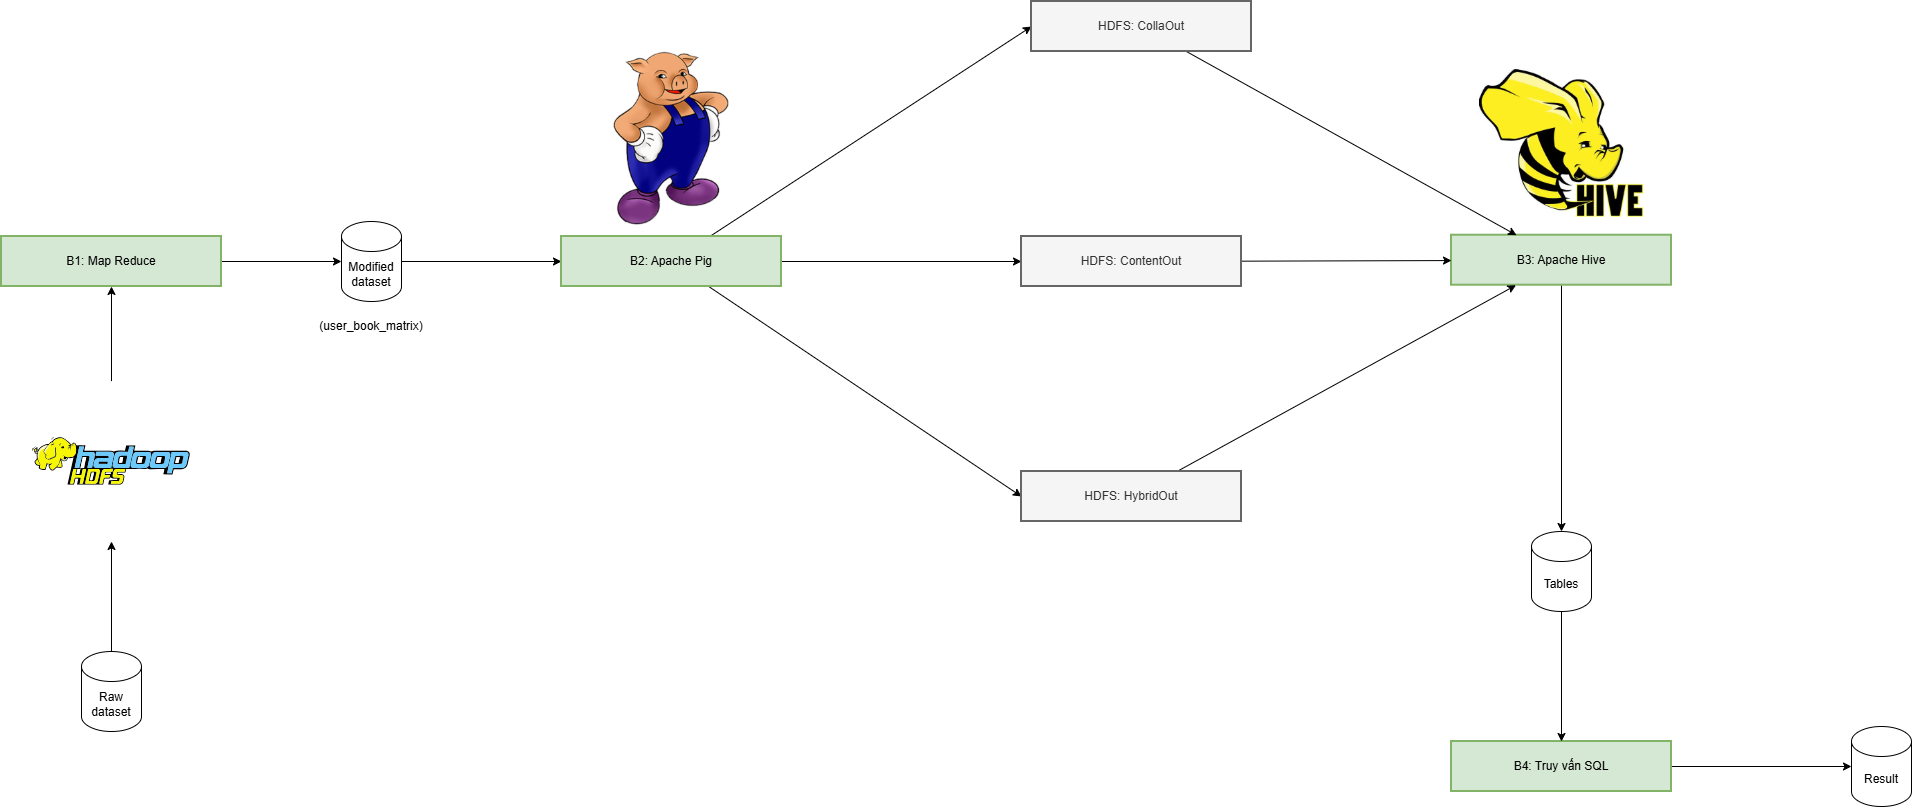
\includegraphics[width=1\textwidth,keepaspectratio]{Images/Big_Data_Flow_Diag.drawio.png}
    \caption{Luồng xử lý tổng quan của hệ thống Book Recommendation}
    \label{fig:workflow_diag}
\end{figure}
